\documentclass{article}
\usepackage{amsmath}
\usepackage{listings}
\usepackage[utf8]{inputenc}
\usepackage{graphicx}
\usepackage{url}
\usepackage{placeins}

\graphicspath{ {../results/} }

\lstset{
	basicstyle=\footnotesize,
	numbers=left,
	tabsize=3,
	title=\lstname,
	breaklines=true
}

\addtolength{\oddsidemargin}{-.875in}
\addtolength{\evensidemargin}{-.875in}
\addtolength{\textwidth}{1.75in}

\addtolength{\topmargin}{-.875in}
\addtolength{\textheight}{1.75in}

\title{Lernverfahren autonomer Roboter - Übung 5}
\author{Tobias Hahn\\ 3073375}	
	
\begin{document}
\maketitle
\newpage
\section*{Übung 5}
\section{Nearest Neighbour Classifier}
\subsection{Distanzmetriken}
Für den Klassifizierer ist es notwendig eine Metrik einzuführen die die Distanz zwischen zwei Punkten als Zahl ermittelt und damit vergleichbar macht. Die drei für die Implementierung verwendeten Distanzmetriken werden im folgenden vorgestellt.
\subsubsection{Normalisierte euklidische Distanz}
Für die normalisierte euklidische Distanz werden die Quadrate der Abstände zwischen den beiden Beispielvektoren für jede Dimension aufsummiert, wobei die Abstände jeweils noch duch die Varianz der Beispiele in dieser Dimension dividiert werden (daher normalisiert). Die Wurzel dieser Summe ist die Distanz. Für das Beispiel wurde die Varianz aus den Beispielen in den Trainingsdaten berechnet und zur Berechnung herangezogen, denkbar ist auch ein Ansatz der dies aus den Testdaten generiert. Jedoch sollten gerade die Testdaten anhand der Trainingsdaten klassifiziert werden, wodurch auch dieser Wert aus den Trainingsdaten kommen sollte.
\paragraph{}
Relevanter Teil des Codes:
\begin{lstlisting}[title=Normalisierte euklidische Distanz]
    (In der Hauptmethode des Klassifizierers)
    sds = np.std(X_train, axis=1)
    distances = [metric(data, compare, sds=sds) for compare in X_train]
    
    (Die Distanzmetrik selber)
    def normalized_euclidean_distance(self, data_a, data_b, **kwargs):
        return np.sqrt(np.sum([(a - b)**2 / sd**2 for a, b, sd in zip(data_a, data_b, kwargs['sds'])]))
\end{lstlisting}

\subsubsection{Chebyshev Distanz}
Eine andere Metrik zur Berechnung der Distanz, welche auch in der Vorlesung vorgestellt wurde, ist die Chebyshev Distanz. Hierbei werden die Beträge der Distanzen der beiden Vektoren betrachtet, wobei sich die Distanz aus der größten Distanz ergibt, also den Abstand der beiden Vektoren in der Dimension darstellt in der dieser am größten ist. 
\paragraph{}
Relevanter Teil des Codes:
\begin{lstlisting}[title=Chebyshev Distanz]
    def chebyshev_distance(self, data_a, data_b, **kwargs):
        return max([abs(a - b) for a, b in zip(data_a, data_b)])
\end{lstlisting}

\subsubsection{Cityblock Distanz}
Die Cityblockdistanz wurde in der Vorlesung nicht vorgestellt, kann jedoch hier\footnote{\url{https://docs.tibco.com/pub/spotfire/6.5.2/doc/html/hc/hc_city_block_distance.htm}} nachgelesen werden. Hierbei werden die Beträge der Abstände zwischen zwei Vektoren für jede Dimension aufsummiert.
\paragraph{}
Relevanter Teil des Codes:
\begin{lstlisting}[title=Cityblock Distanz]
    def cityblock_distance(self, data_a, data_b, **kwargs):
        return np.sum([abs(a - b) for a, b in zip(data_a, data_b)])
\end{lstlisting}

\subsection{Accuracy}
Der implementierte Klassifizierer wurde am bekannten Irisdatenset geprüft, wobei der Parameter für die Anzahl der betrachteten Nachbarn von 1 bis 100 variiert wurde. Dieser Parameter gibt an die wieviel nächsten Punkte des betrachteten Punktes zur Klassifizierung verwendet werden, wobei die Klassenlabel betrachtet werden. Das Klassenlabel das in den Daten am öftesten vorkommt wird verwendet. Die Nähe wird dabei durch die normalisierte euklidische Distanz angegeben.

\subsubsection{Plot}
Die Resultate sind in folgendem Plot zu sehen:
\begin{figure}[h]
    \centering
    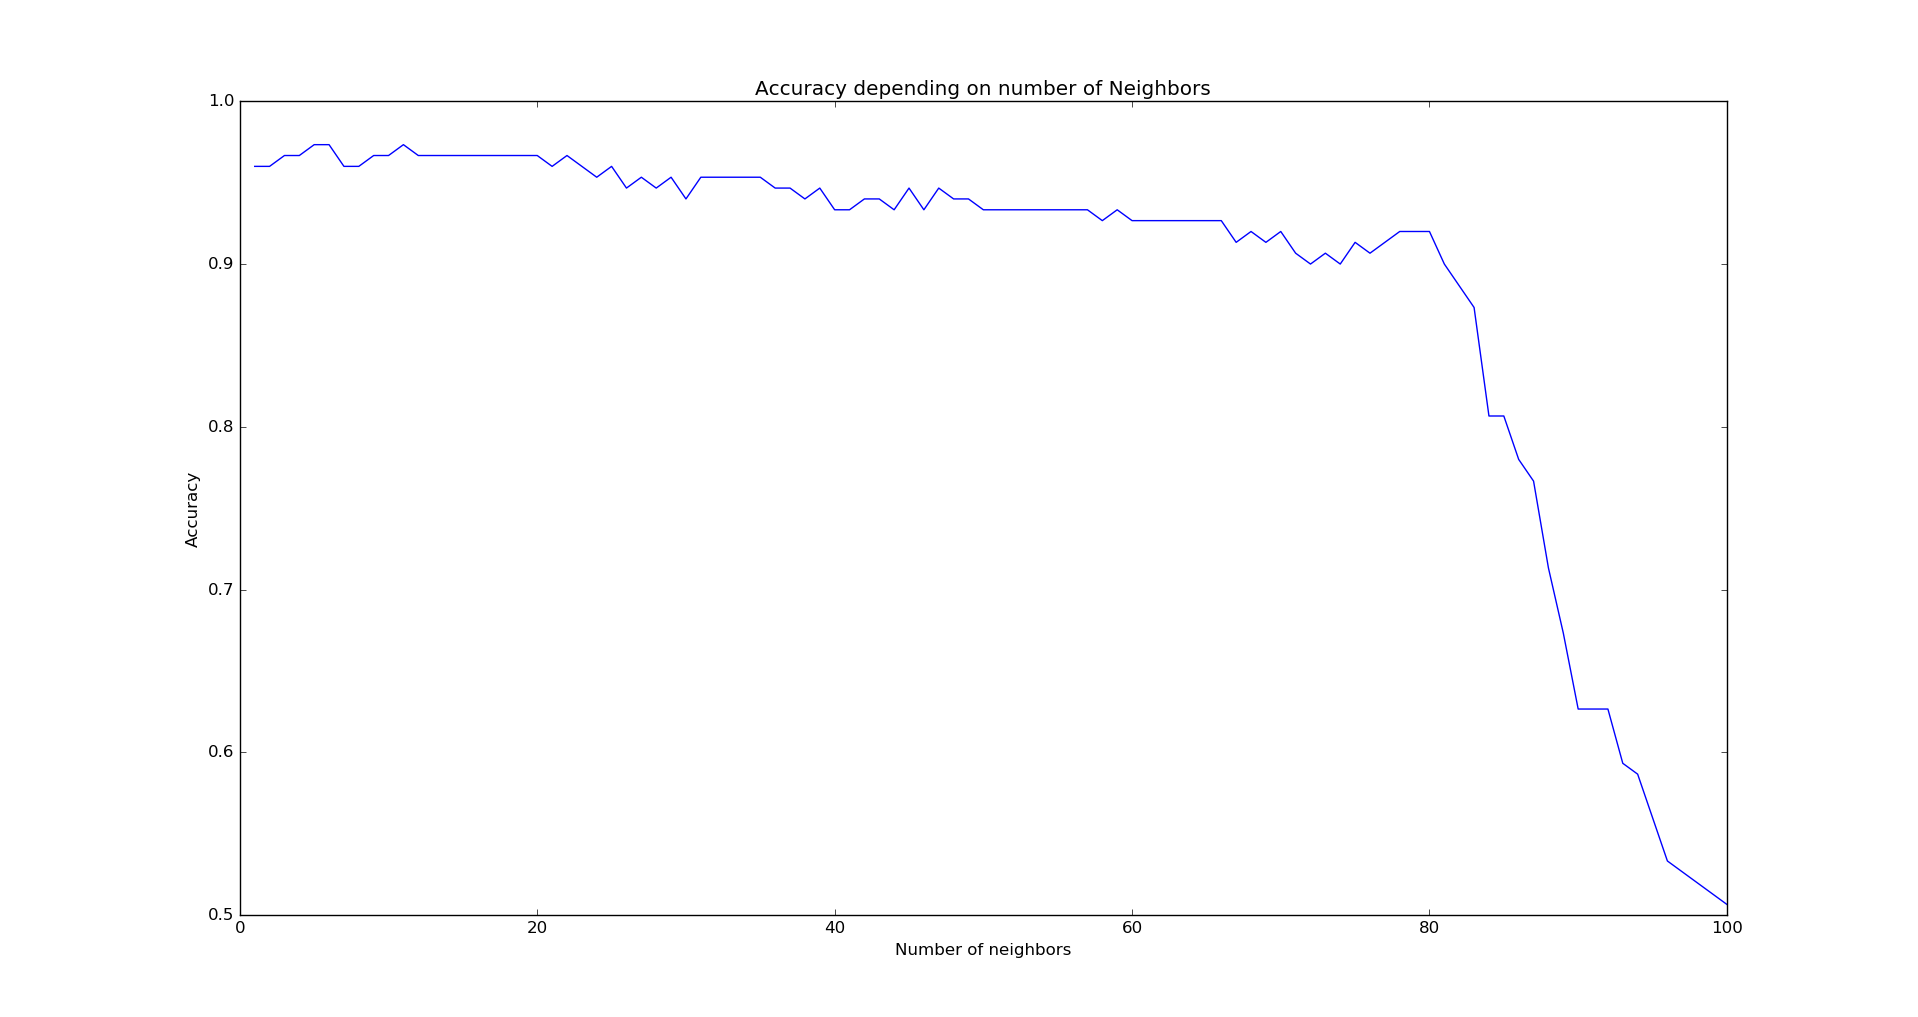
\includegraphics[width=\textwidth]{euclidean.png}
    \caption{Die Accuracy zu der verwendeten Anzahl von Nachbarn}
    \label{fig:euc}
\end{figure}
\FloatBarrier
\subsubsection{Erklärung}
Wie man sehen kann bleibt die Accuracy bis zu einer gewissen hohen Anzahl an Nachbarpunkten (80+) relativ stabil, wobei das Maximum bei 5 erreicht ist und danach ein leichter Abstieg stattfindet. Über 80 nimmt die Accuracy rapide ab, bis sie bei 100 Nachbarn bei annähernd 0.5 landet.
\paragraph{}
Die relative Stabilität bis 80 lässt sich dadurch erklären, dass die Punkte der drei Labelcluster relativ gut getrennt sind. Daher bleiben auch die Nachbarn mit richtigem Label in der Tendenz in der Mehrzahl, wenn man mehr Nachbarn betrachtet. Der rapide Abfall nach 80 ist dadurch erklärbar, dass bei so einer hohen Anzahl an Nachbarn die Wahrscheinlichkeit dass ein Punkt als Nachar in Betracht gezogen wird fast Unabhängig von seiner Entfernung wird, die Häufigkeit der Label in der Nachbarschaft sich der Verteilung der Label in der Grunddatenmenge annähert. Dadurch wird die Klassifizierung mehr zu einer Aussage darüber welches Label am öftesten in der Datenmenge vorkommt, anstatt etwas zur Klassenzugehörigkeit zu sagen: Kleiner Cluster haben gar keine Mitglieder mehr, während größere Cluster viel zu viele haben.

\subsection{Andere Distanzmetriken}
Der gleiche Versuch wurde auch mit anderen Distanzmetriken gestartet. Die Versuche ähneln sich sehr stark, wie man an den folgenden beiden Plots sieht:

\subsubsection{Plot}
Die Resultate sind in folgenden Plots zu sehen:
\begin{figure}[h]
    \centering
    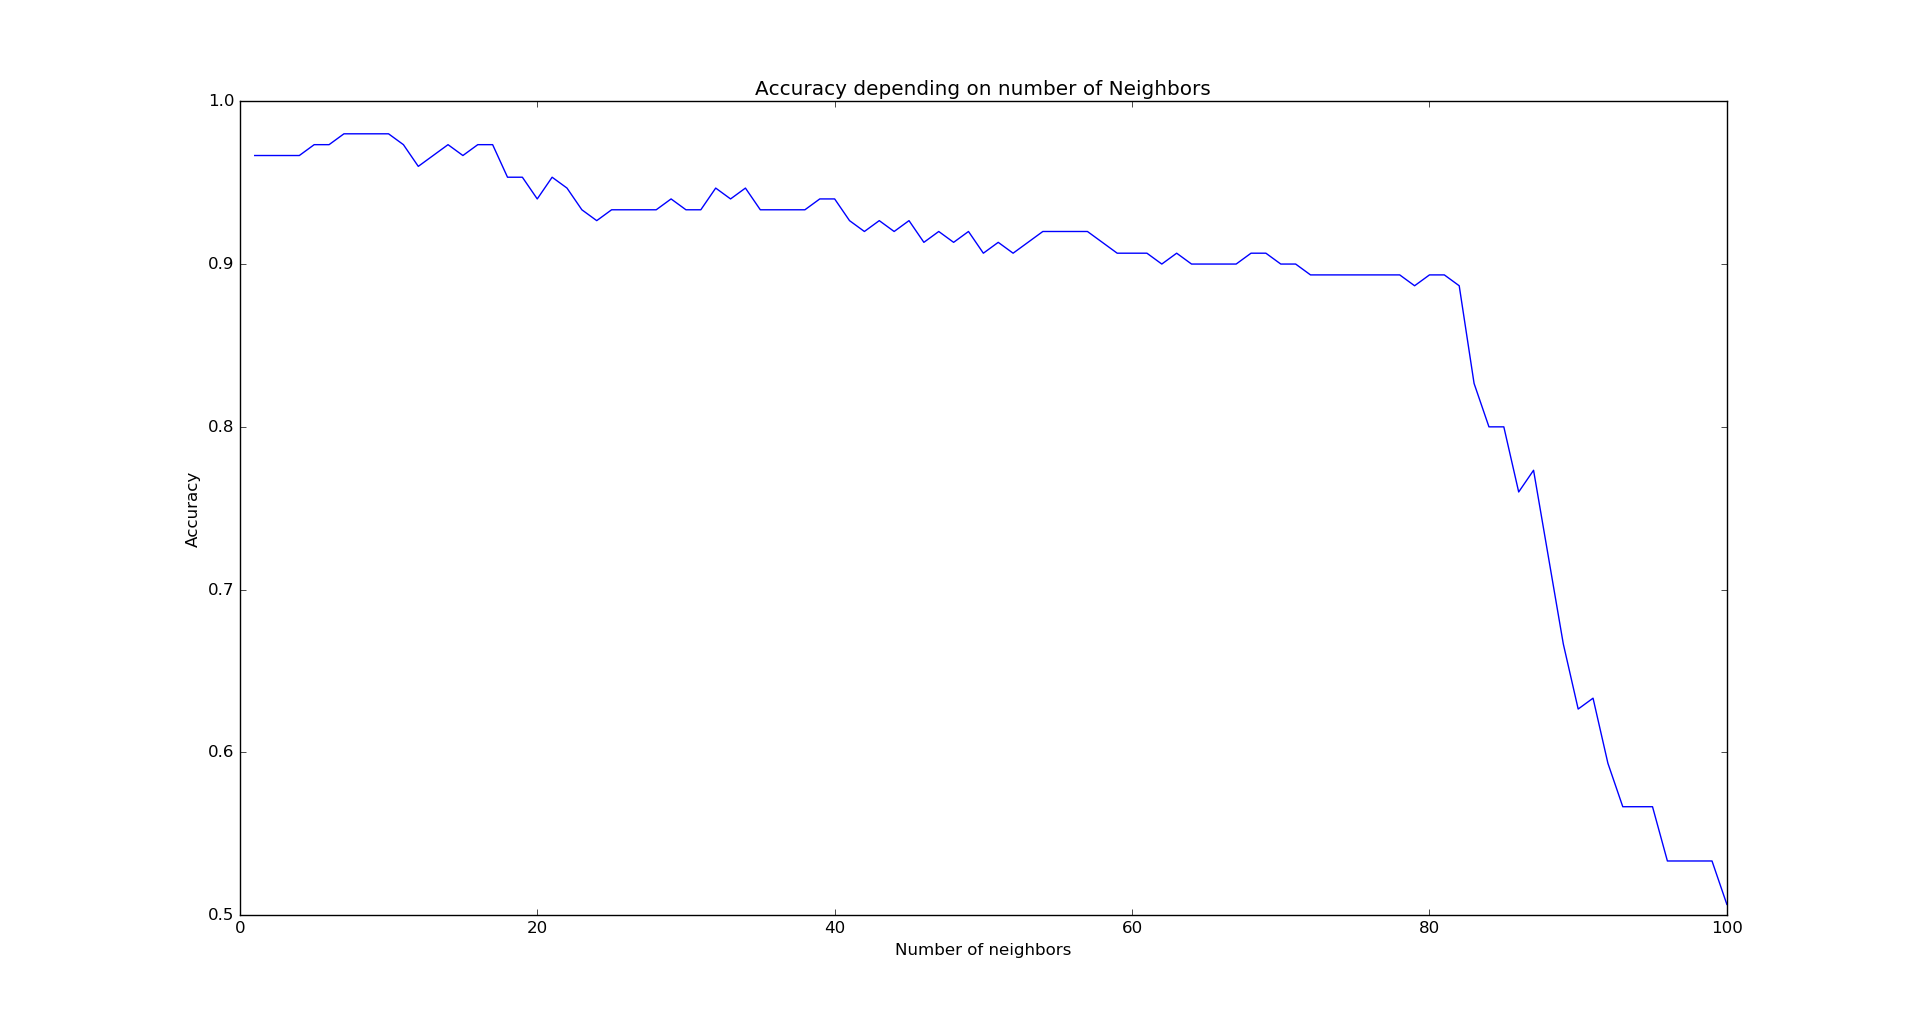
\includegraphics[width=0.8\textwidth]{chebyshev.png}
    \caption{Die Accuracy zu der verwendeten Anzahl von Nachbarn mit Chebyshev Distanz}
    \label{fig:cheby}
\end{figure}

\begin{figure}[h]
    \centering
    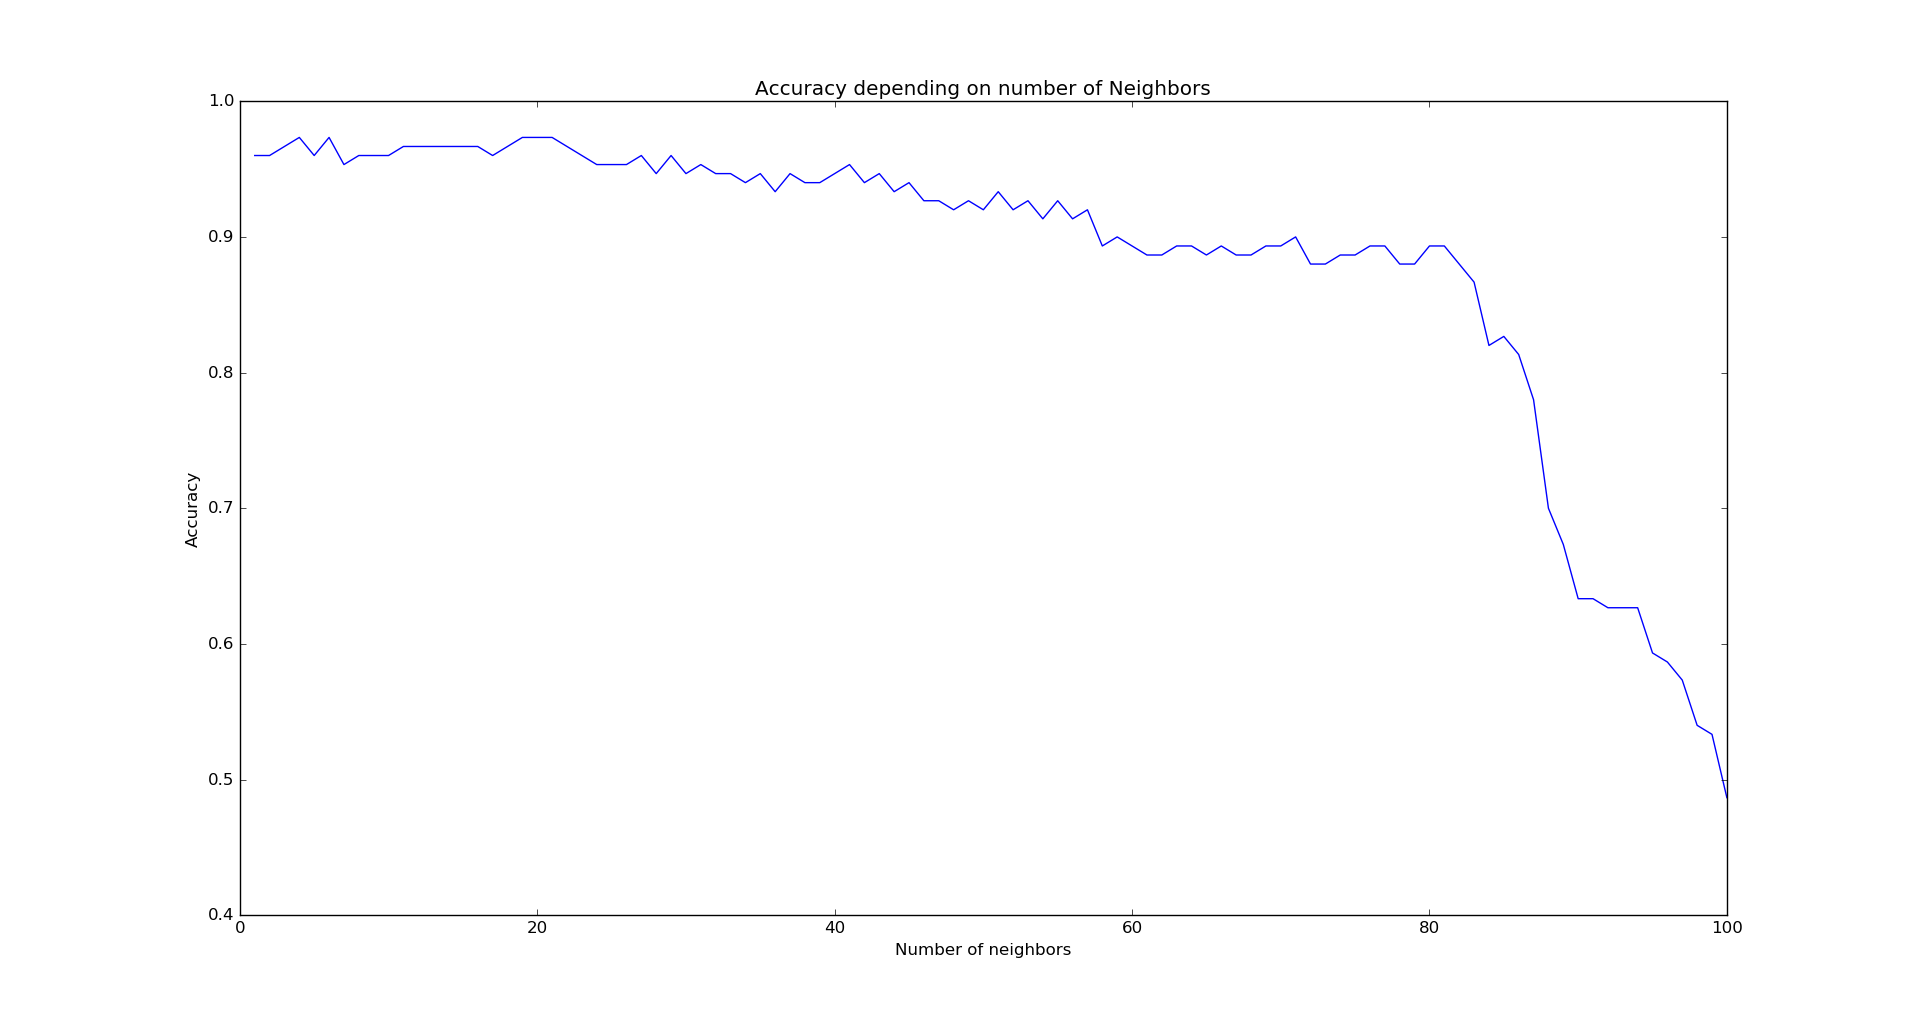
\includegraphics[width=0.8\textwidth]{cityblock.png}
    \caption{Die Accuracy zu der verwendeten Anzahl von Nachbarn mit Cityblock Distanz}
    \label{fig:city}
\end{figure}
\FloatBarrier
\subsubsection{Erklärung}
Wie man sieht ist die Accuracy ziemlich identisch. Dies liegt daran dass alle drei Distanzmetriken auf dem Abstand der Punkte im Raum abhängen, und daher die ähnlichen Argumente wie bei Punkt Zwei zutreffen.

\end{document}
